\documentclass{article}
\usepackage[utf8]{inputenc}
\usepackage[spanish]{babel}
\usepackage{graphicx, graphics, float}
\usepackage[a4paper, total={6in, 10in}]{geometry}
\title{DSD Memoria Práctica 3}
\author{Andrés Merlo Trujillo}
\date{}
\begin{document}
%TODO: MUY IMPORTANTE COMPROBAR LOS DE LAS INSTANCIAS DEL SERVIDOR, SEGURAMENTE ESTE MALY SE REFIERA A INSTANCIAS DEL METODO REMOTO O ALGO
%TODO 2: PLANTEAR EN ELIMINAR EL APARTADO DE IMPLEMENTACION YA QUE APARECE EN EL PDF
%TODO 3: QUIZAS PONER LOS METODOS QUE SE MENCIONAN EN LA PARTE 2 COMO UNA LISTA
%TODO 4: EXPLICAR UN POCO MAS LA PALABRA CLAVE SYNCHRONIZED
\maketitle

\section{Primera parte, Ejemplos}
En esta primera parte se pide copiar los códigos de prueba que aparecen en el guión de prácticas y comentar como funcionan y qué hacen.

\bigskip

Lo primero que hay que hacer es tener instalado una versión de OpenJDK lo suficientemente antigua porque si no al usar el comando \textit{javac *.java} saldrá un error similar a este:

%INSERTAR ERROR DE COMPILACIÓN

En mi caso tenía la versión 18 de JDK y he tenido que descargarme la versión 11 de la misma y configurarla para que sea la que se use por defecto.

\bigskip

Algo interesante que me ha ocurrido (no sé si ha sido mucha casualidad, pero he probado la ejecución varias veces) es que estaba usando la versión de JDK 8 y en la primera parte del ejemplo 2 se daba bien la ejecución de las hebras sin haber entrelazamientos y sin usar la palabra clave \textit{synchronized}. Como me extrañaba, probé la última versión que tenía disponible mi distribución antes de dar error de compilación, que en este caso es la versión 11, como he dicho anteriormente. Con la versión 11 si se producen entrelazamientos, por lo que supongo que es problema de la versión.

\bigskip
%QUIZAS HAGA FALTA ELIMINAR ESTO
Otro problema que he tenido esa la hora de usar el script, ya que dentro del mismo se lanzan secuencialmente el servidor y los clientes, esto produce que se lancen nada más que el servidor y que los clientes no se lancen.

%FOTO DE LO OCURRIDO
Para ello he separado la parte de la invocación de los clientes en otro script para poder lanzar ambos en dos terminales distintas.

\subsection{Ejemplo 1}
\subsubsection{Descripción}
Este ejemplo lo que realiza en el lado del cliente es llamar al método remoto \textit{escribir\_mensaje} con el identificador pasado por consola del cliente.

En el lado del servidor al ejecutar el método hay dos opciones, si el identificador pasado acaba en 0 entonces duerme durante 5000 ms (5 segundos), en otro caso simplemente indica que ha recibido la petición y muestra el identificador del cliente.

%FOTO CON ALGUNA EJECUCION
\begin{figure}[H]
    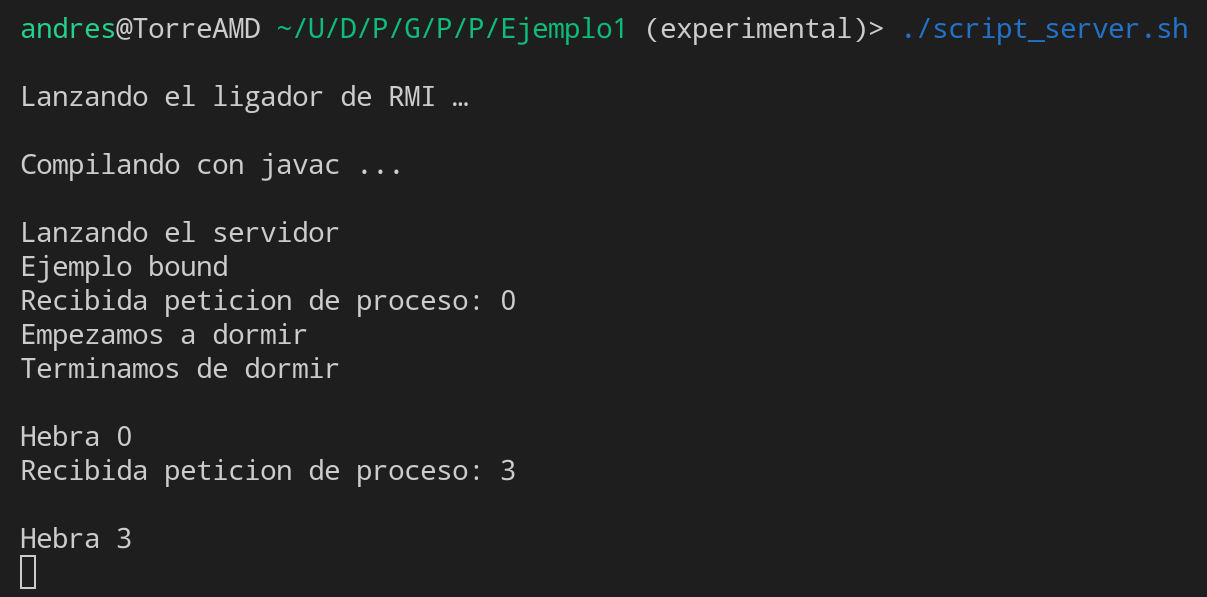
\includegraphics[width=\textwidth]{imagenes/E1S.png}
    \caption{Salida del servidor al ejecutar los clientes}
\end{figure}

Como se puede observar el primer cliente que se lanza tiene el identificador 0, por lo que se pone a dormir y se indica en el servidor. El siguiente, que tiene identificador 3, simplemente hace que se muestre en el servidor su información, pero no se duerme.

\begin{figure}[H]
    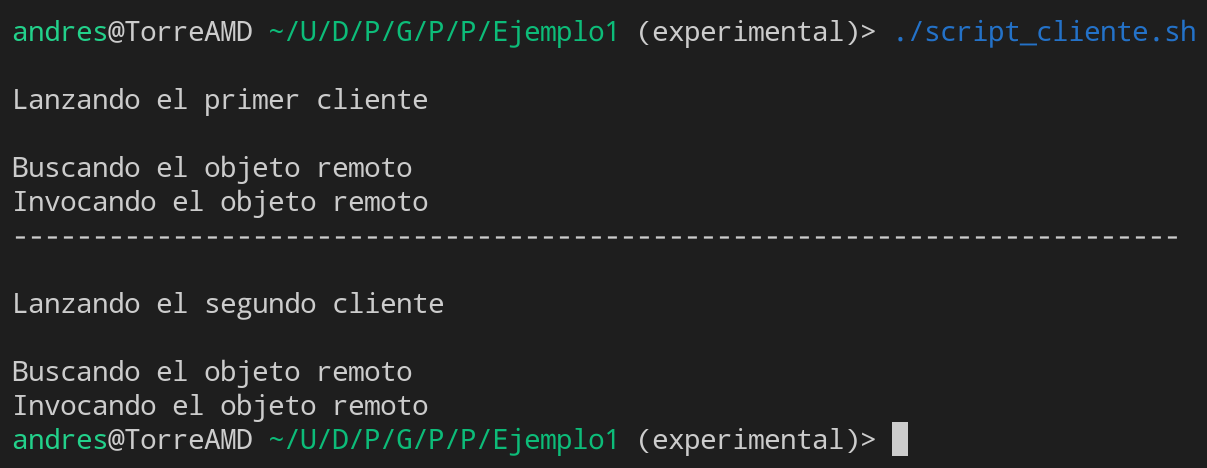
\includegraphics[width=\textwidth]{imagenes/E1C.png}
    \caption{Salida de los clientes}
\end{figure}

\subsubsection{Implementación}
Para la implementación de este sistema primero es necesario realizar la interfaz remota del servidor que va a exportar los métodos a los clientes. En este caso solo se exporta el método \textit{escribir\_mensaje}.

En la parte del servidor se crea una clase que implementa los métodos de la interfaz remota ``Ejemplo\_I''.

El método imprime por la pantalla del servidor (remota) que ha recibido la petición del proceso. Además comprueba si el número de proceso es 0, en caso afirmativo se manda el cliente que ha llamado al método remoto a dormir durante 5 segundos y luego, con independencia de que sea el proceso 0 ó no, se indica el identificador del cliente en la pantalla remota.

En la parte del main del servidor activa el gestor de seguridad, que es exactamente igual para el cliente, crea una instancia de del objeto remoto y por último se exporta y se registra en ``rmiregistry'' para que los clientes puedan encontrarlo.

En la parte del cliente se activa el gestor de seguridad accede al ``rmiregistry'' que se encuentra en la dirección pasada por consola, y obtiene a partir del registro el stub del objeto remoto para poder lanzar el método anteriormente mencionado.


\subsubsection{Funcionamiento}
El diagrama del sistema (sin incluir rmiregistry ni stubs, solo los propios objetos y clases) es el siguiente:

\begin{figure}[H]
    \centering
    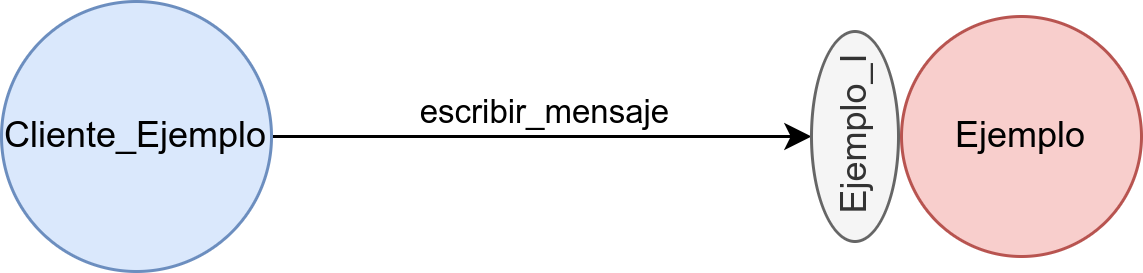
\includegraphics[width=0.5\textwidth]{imagenes/E1Diagrama.png}
    \caption{Diagrama con las comunicaciones que se realizan}
\end{figure}

Se puede ver que el cliente llama al método escribir\_mensaje exportado por la interfaz remota del servidor, que se llama Ejemplo.

\subsection{Ejemplo 2}
\subsubsection{Descripción}
En este ejemplo se realiza algo similar al anterior, pero esta vez el cliente lanza un número de hebras que se pasan por consola. La lógica del servidor es exactamente igual al ejemplo anterior (y la del cliente también, pero es con hebras).

\textbf{¿Se entrelazan los mensajes?: }Sí existe entrelazamiento. Tras varias ejecuciones se puede observar como se produce un entrelazamiento de mensajes de salida en el servidor en el que se muestra que entran varias hebras a la vez antes de que la primera haya mostrado el mensaje de salida y luego cuando salen muestra varias veces también el mensaje de salida. Puede que esto sea algo no deseado y que siempre se desee que las hebras siguientes esperen a que la hebra que va delante reciba la respuesta del servidor para que siempre haya como mucho una hebra en el método remoto.

\begin{figure}[H]
    \centering
    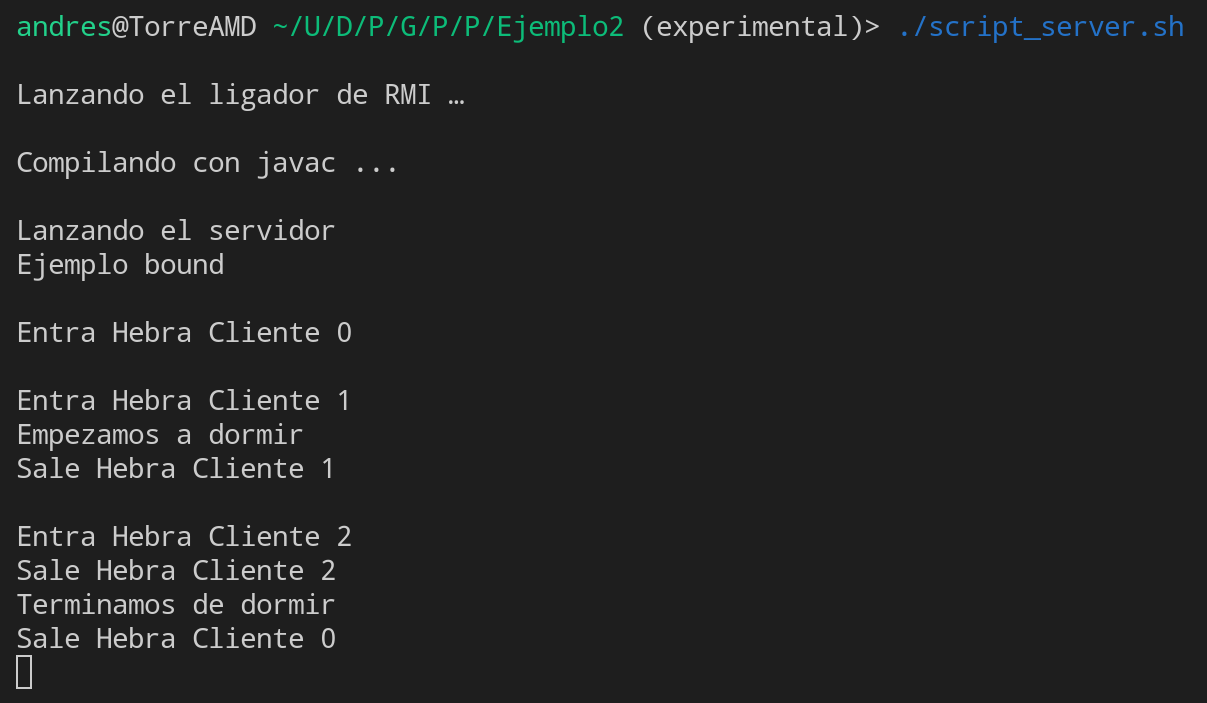
\includegraphics[width=0.7\textwidth]{imagenes/E2Server1.png}
    \caption{Entrelazamiento entre los mensajes de la hebra cliente 0 y 1}
\end{figure}

\begin{figure}[H]
    \centering
    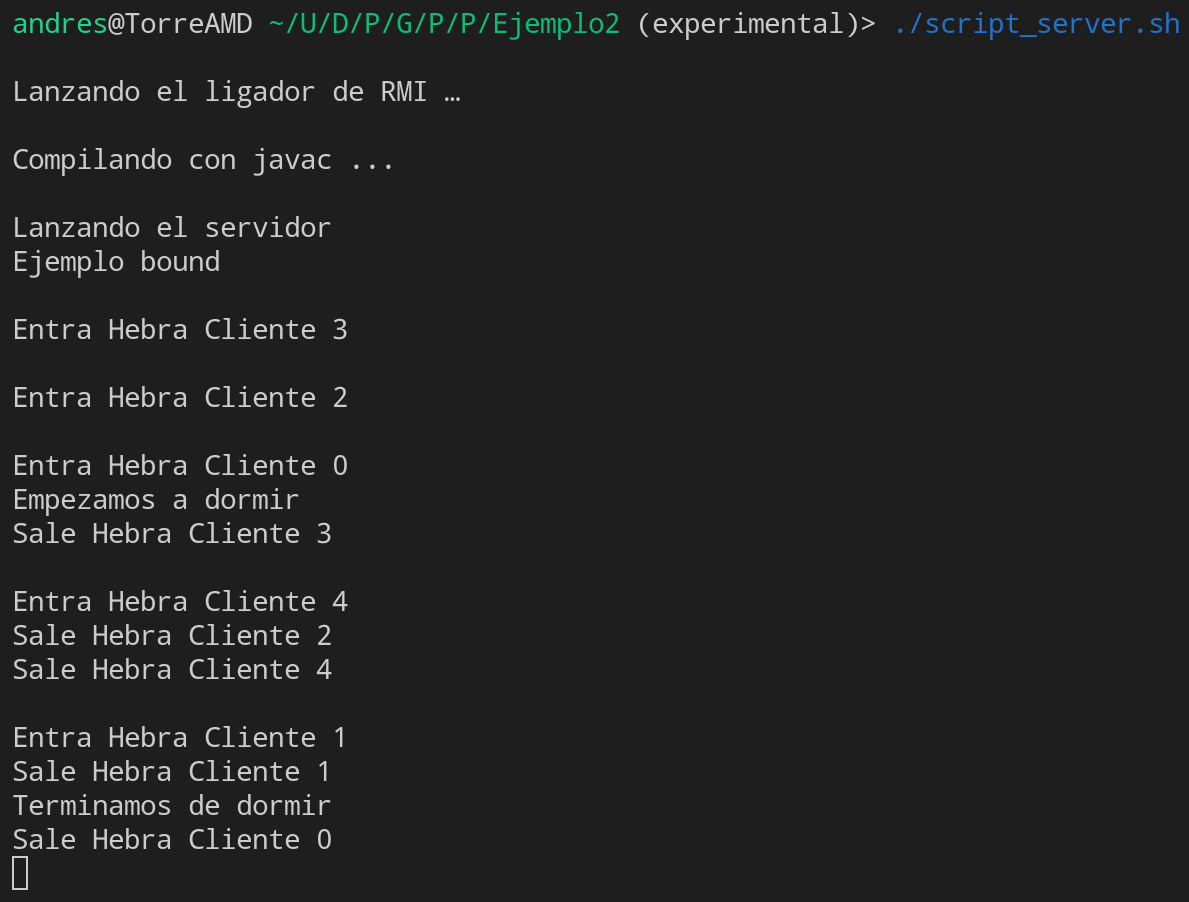
\includegraphics[width=0.7\textwidth]{imagenes/E2Server2.png}
    \caption{Entrelazamiento entre los mensajes de las hebras 0, 2, 3 y 4.}
\end{figure}

Otro entrelazamiento menor que ocurre es que las hebras no realizan las peticiones de manera ordenada al servidor; es decir, en la impresión que realiza el servidor por consola se puede observar que no siguen un orden ascendente los identificadores de los clientes. Puede ser porque realmente las hebras del cliente no llamen al método remoto en el mismo orden en que se crean (las hebras). Esto se puede ver en la imagen anterior.

\bigskip

\textbf{¿Qué hacen las demás hebras?: }Las demás hebras no esperan a que la hebra de delante reciba la respuesta del método remoto haciendo que el servidor esté ejecutando el mismo método concurrentemente produciendo así, como se ha dicho anteriormente, entrelazamientos.  
Esto implica que si el método tuviera una sección crítica, por ejemplo una escritura a una variable, se podría producir en algún entrelazamiento una condición de carrera invalidando el valor de la variable, que debería haber sido atómica. Es por eso que es necesario aplicar técnicas de sincronización (cerrojos, semáforos, monitores, etc.) entre clientes/hebras para un correcto estado del objeto que exporta el servidor.

%MOSTRAR TAMBIEN UNA FOTO SOBRE ESO
%MOSTRAR UN DIAGRAMA CON LOS POSIBLES ENTRELAZAMIENTOS, POR EJEMPLO HACER PARA EL CASO DE 3 HEBRAS
Por ejemplo, para el caso de 2 hebras se podrían dar los siguientes entrelazamientos de mensajes (supongo que son la hebra 1 y 2 para evitar entrelazamientos especiales con el bloqueo de la hebra 0):

\begin{center}
    \centerline{
        \begin{tabular}{ | c | c | c | c | c | c | }
            \hline
            Entra Hebra 1 & Entra Hebra 1 & Entra Hebra 1 & Entra Hebra 2 & Entra Hebra 2 & Entra Hebra 2 \\
            Sale Hebra 1 & Entra Hebra 2 & Entra Hebra 2 & Entra Hebra 1 & Entra Hebra 1 & Sale Hebra 2 \\
            Entra Hebra 2 & Sale Hebra 1 & Sale Hebra 2 & Sale Hebra 2 & Sale Hebra 1 & Entra Hebra 1 \\
            Sale Hebra 2 & Sale Hebra 2 & Sale Hebra 1 & Sale Hebra 1 & Sale Hebra 2 & Sale Hebra 1 \\
            \hline
        \end{tabular}
    }
\end{center}

\textbf{¿Qué ocurre con las hebras cuyo nombre acaba en 0?: }Las hebras que acaban en 0, al igual que en el ejemplo 1, se ponen a dormir durante 5000 ms (5 segundos) al llamar al método remoto. Durante ese tiempo, otras hebras pueden invocar al método remoto para su ejecución y este se ejecuta paralelamente a los otros, como se ha mencionado anteriormente. Esto hace que pueda haber instancias en el servidor que estén durmiendo e instancias que se estén ejecutando concurrentemente.

\subsubsection{Implementación}
La implementación de la parte del servidor es exactamente igual que en el ejemplo 1, salvo por algún ligero cambio del mensaje que se muestra por pantalla.


%ESTA ULTIMA PARTE ES NECESARIA COMPROBARLA
En la parte del cliente se realiza prácticamente lo mismo, pero se encapsula en el método \textit{run}, ya que son hebras, luego desde el main se crea un array de hebras y se lanzan con \textit{start}.

\subsubsection{Uso de \textit{synchronized}}
Cuando se añade la palabra clave \textit{synchronized} al método remoto del servidor ya no se produce entrelazamientos. Sin embargo las hebras que acaban en 0 se ponen a dormir y bloquea al servidor para recibir más peticiones al mismo método produciendo así posibles esperas innecesarias. Según la documentación, cuando más de una hebra llama a métodos que tienen \textit{synchronized}, solo entra uno de ellos y los demás se quedan bloqueados esperando a que salga el de delante. Esto implica que el bloqueo no solo se puede dar en una llamada a un método en concreto, sino también en varios métodos con esta palabra clave.

\begin{figure}[H]
    \centering
    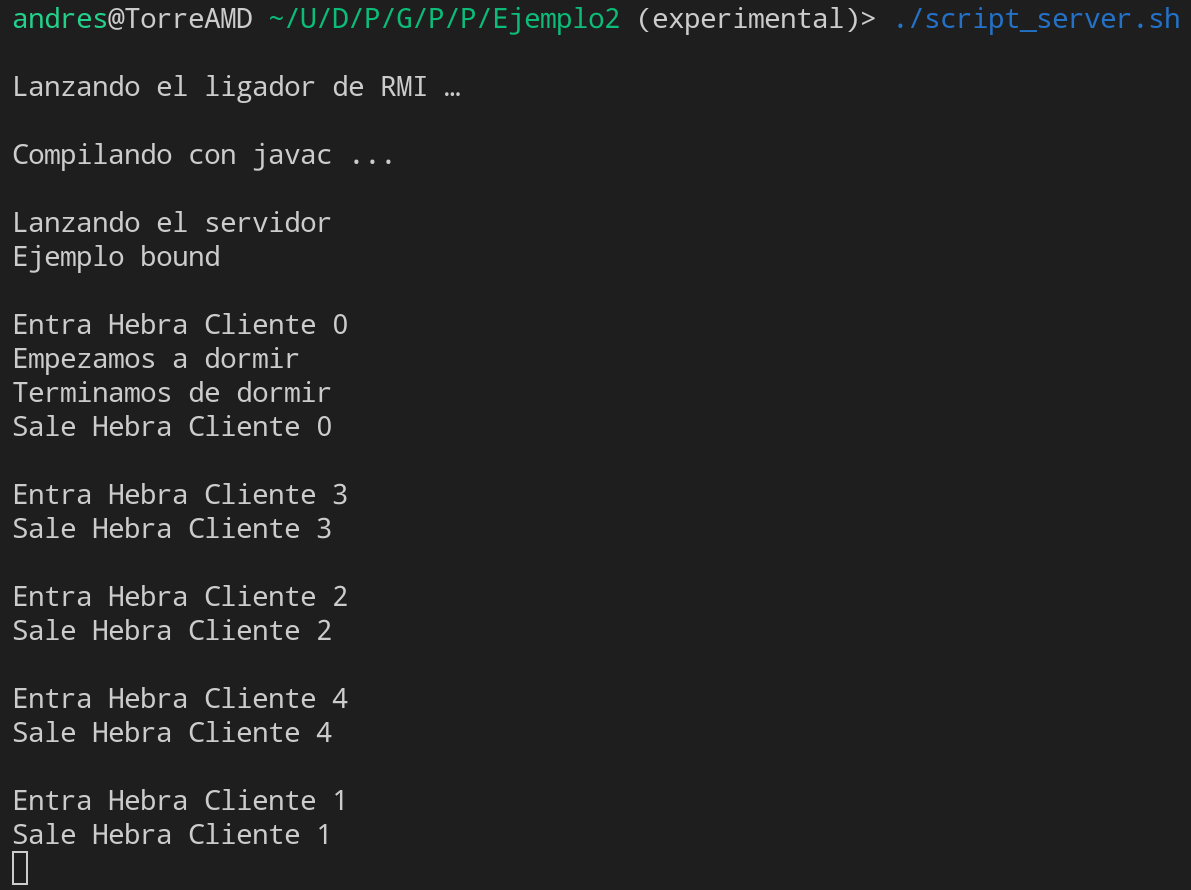
\includegraphics[width=0.7\textwidth]{imagenes/E2ServerSync1.png}
    \caption{Salida por pantalla del servidor.}
\end{figure}

Como se puede observar, la hebra 0 empieza a dormir y las demás hebras no pueden ejecutar el método hasta que se cumpla el periodo de dormir. Esto arreglaría el entrelazamiento, pero a costa de introducir esperas innecesarias, ya que ahora el método se comporta como si fuera monohebrado.

Como conclusión se puede decir que la principal diferencia entre no usar \textit{synchronized} y sí usarlo es que en el primero las hebras no necesitan esperar a que salgan las de delante para que su petición pueda ser procesada. Mientras que en el segundo caso solo una hebra puede acceder a métodos \textit{synchronized} y las demás tienen que esperar su finalización para que puedan acceder.

\begin{figure}[H]
    \centering
    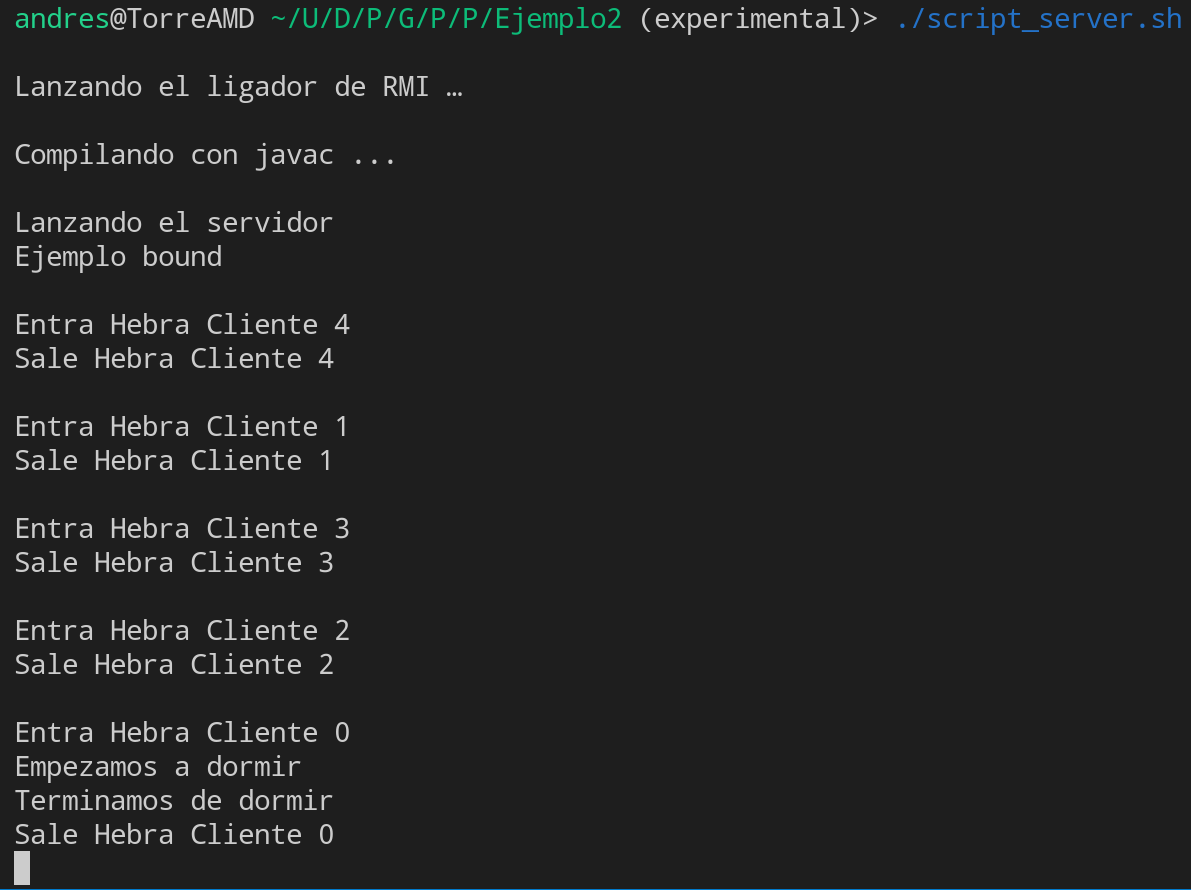
\includegraphics[width=0.7\textwidth]{imagenes/E2ServerSync2.png}
    \caption{Otra salida por pantalla del servidor.}
\end{figure}

Por último, el diagrama de la relación entre objetos es el siguiente (como antes, obviando stubs y rmiregistry):

\begin{figure}[H]
    \centering
    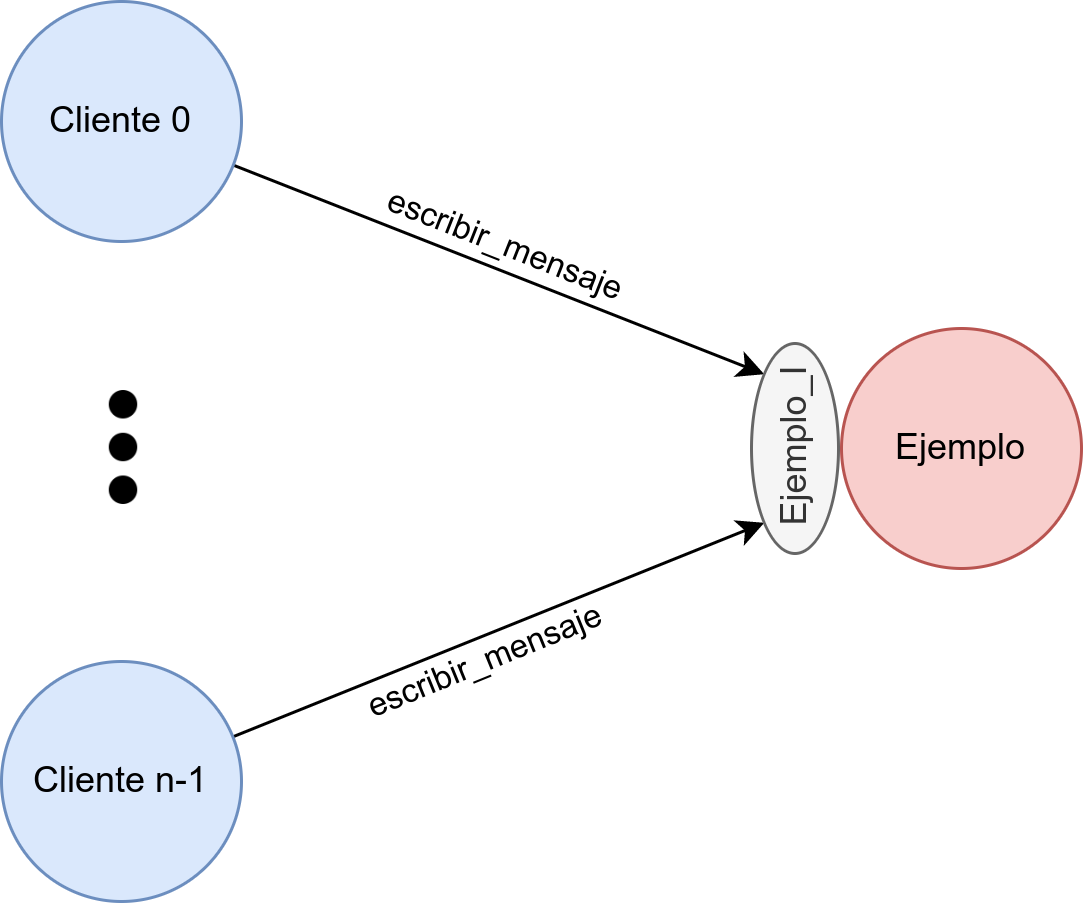
\includegraphics[width=0.5\textwidth]{imagenes/E2Diagrama.png}
\end{figure}

\subsection{Ejemplo 3}
\subsubsection{Descripción}
En este ejemplo se separa el propio objeto remoto del servidor. Para ello se crea la interfaz remota como en los ejemplos anteriores, pero esta vez se implementa en una clase aparte sin tener un main asociado.

El main se encuentra en otra clase servidor que se encarga como en los demás ejemplos de crear la instancia del objeto remoto y exportarlo al \textit{rmiregistry}.

\bigskip

Por la parte del cliente realiza la misma tarea que en los ejemplos anteriores, pero esta vez una vez creado el stub pone el contador a 0, ya que es posible que otros procesos hayan modificado el atributo ``suma''. Una vez realizado esto toma el tiempo de entrada y realiza 1000 llamadas al método remoto \textit{incrementar}, cuando acaba de realizar las llamadas toma el tiempo de salida y muestra por consola el tiempo que ha tardado y, haciendo una llamada al método getter remoto \textit{sumar}, obtiene el valor del atributo del objeto remoto, que en caso de no haber sido accedido por otros procesos o hebras será el mismo número que el de llamadas RMI realizadas, que es 1000.

%MOSTRAR IMAGEN DE ESTO Y QUIZAS AÑADIR ALGO MAS

\begin{figure}[H]
    \centering
    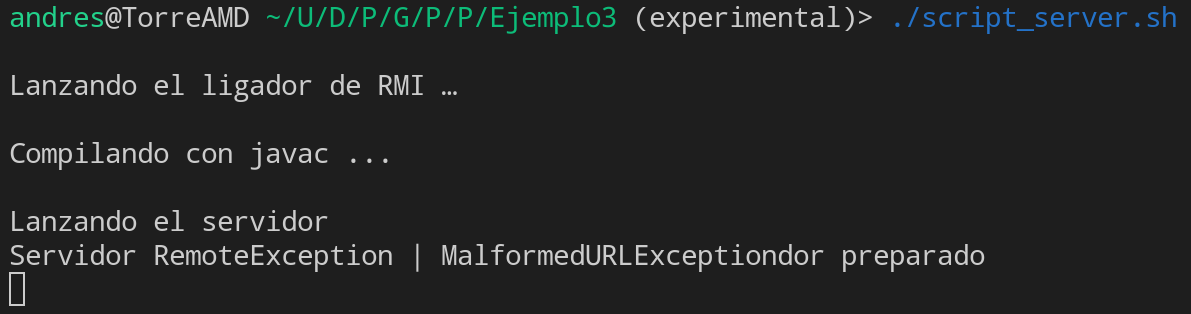
\includegraphics[width=0.7\textwidth]{imagenes/E3S1.png}
    \caption{Salida por pantalla del servidor}
\end{figure}

\begin{figure}[H]
    \centering
    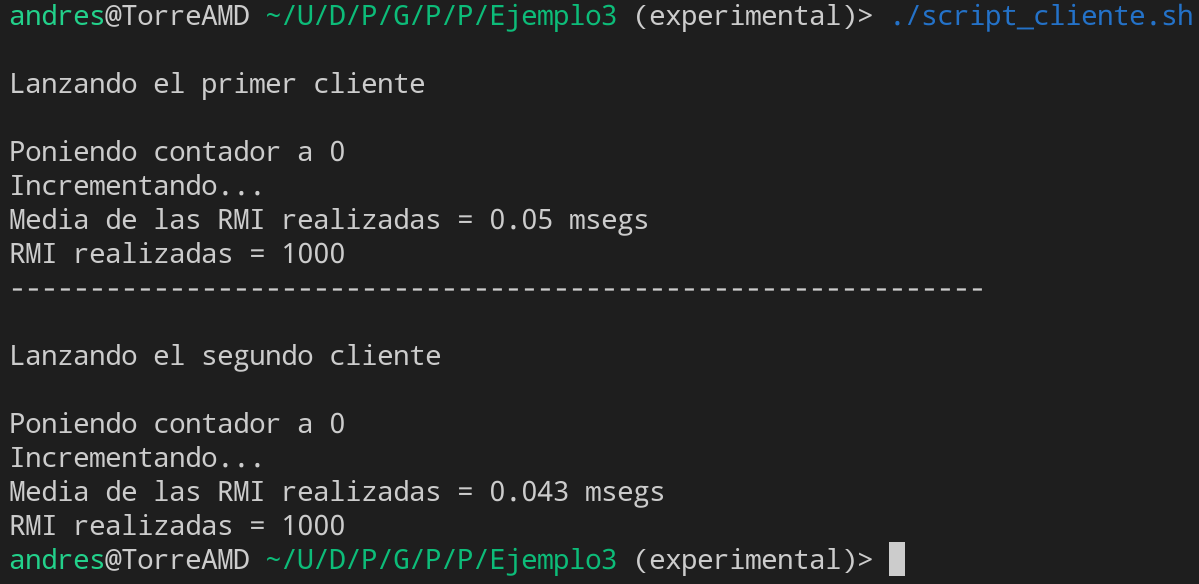
\includegraphics[width=0.7\textwidth]{imagenes/E3C1.png}
    \caption{Salida por pantalla de los clientes (delimitados por ``-'')}
\end{figure}

Por último, como en los ejemplos anteriores, un diagrama con las relaciones entre objetos:

\begin{figure}[H]
    \centering
    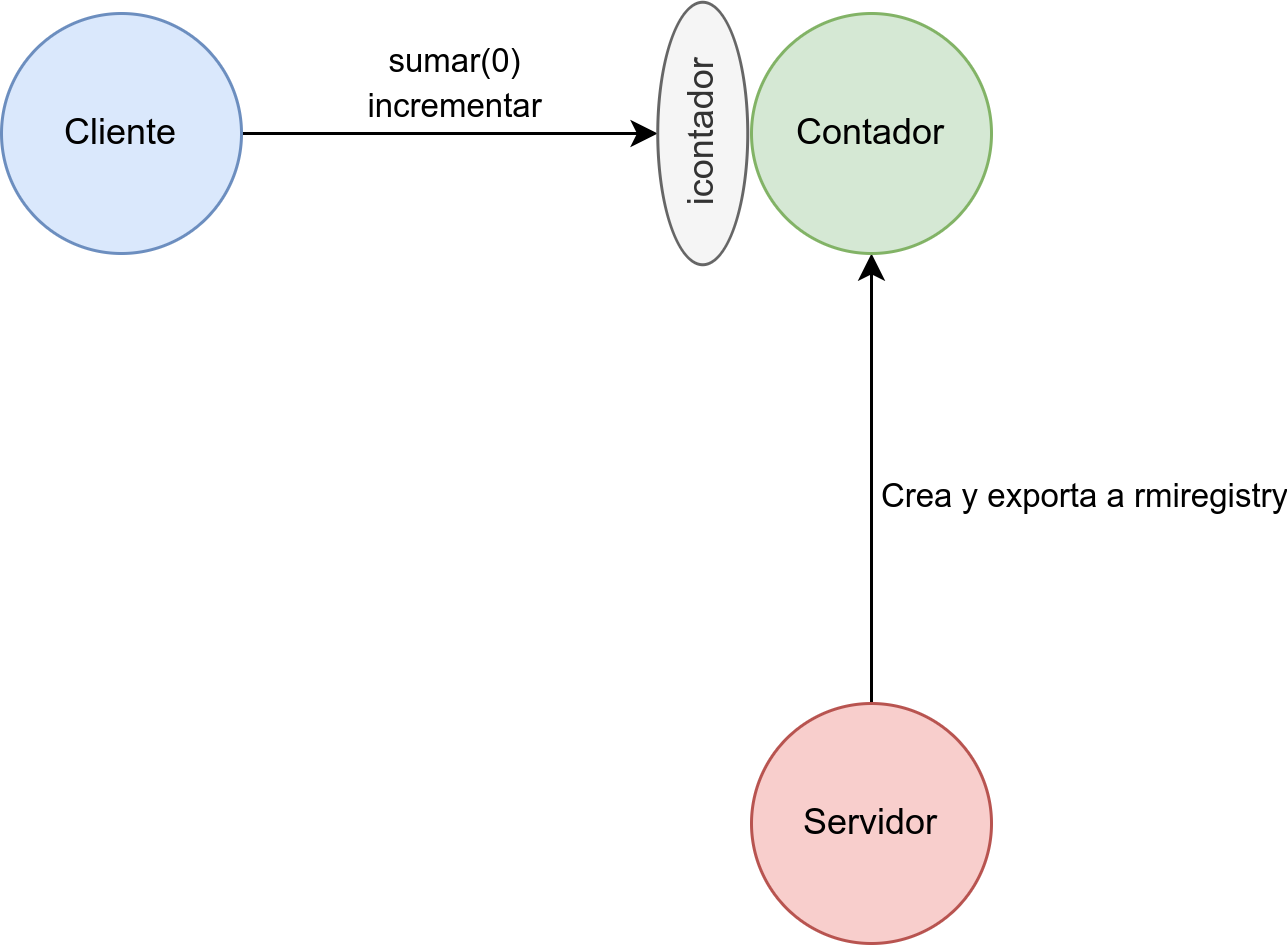
\includegraphics[width=0.5\textwidth]{imagenes/E3Diagrama.png}
\end{figure}

\subsection{Diferencias entre los ejemplos}
En estos 3 ejemplos se han visto varios aspectos importantes de RMI que hace que los diferencien en cierta medida. 

La primera diferencia es que en los ejemplos 1 y 3 se usan solamente los procesos como tal en los que no existen hebras, sino los propios procesos (JVM). Mientras que en el ejemplo 2 el cliente lanza varias hebras que acceden concurrentemente a un método remoto.

La segunda diferencia es en la implementacion de la interfaz remota, en la que en los ejemplos 1 y 2 se realiza en la propia clase del servidor mientras que en el ejemplo 3 se realiza en una clase aparte, haciendo que el servidor solo se encargue de crear la instancia remota y exportarla. Esto permite separar la implementación del objeto remoto del propio código del servidor.

Otra diferencia se encuentra en el uso de \textit{rmiregistry}, el servidor en los ejemplos 1 y 2 supone que se ha lanzado el rmiregistry y solo se encarga en exportar el objeto remoto, mientras que en el ejemplo 3 es el propio servidor el que crea el rmiregistry y le asigna un puerto mediante el método \textit{createRegistry}, es más, si se intenta lanzar rmiregistry primero y luego este servidor va a dar error por lo que es necesario matar a todos los procesos que el sistema tenga.

%MOSTRAR EL ERROR EXPLICADO EN EL PARRAFO ANTERIOR

\section{Segunda parte, servidor de donaciones}
\subsection{Descripción}
En esta parte de la práctica se pide realizar un servidor de donaciones replicado y balanceado al que los clientes se conectarán para realizar donaciones. Cuando un cliente nuevo se registre en cualquiera de las réplicas le asignará la réplica correspondiente que tenga menos usuarios suscritos.

Adicionalmente, se pueden añadir métodos nuevos con funcionalidad distinta o arreglar el problema de la exclusión mutua con alguno de los algoritmos vistos en clase de teoría.

\subsection{Implementación parte obligatoria}
Para implementarlo he decidido realizar dos interfaces remotas para el servidor de donaciones: una primera que servirá para la interconexión entre réplicas y otra que usarán los clientes para comunicarse con estas réplicas.

%MOSTRAR DIAGRAMA DE LAS REPLICAS CON LAS INTERFACES

La clase ``Servidor'' (la réplica) implementa estas dos interfaces más algunos métodos internos que no son necesarios ser exportados por ninguna interfaz.

Esta clase consta de un atributo estático (de clase) que contiene el número de réplicas que se han instanciado, ya que en mi caso he supuesto que puede haber un número arbitrario de réplicas. También contiene otro atributo estático que es el total donado por todos los clientes de todas las réplicas.

Luego cada réplica tiene su propio identificador numérico y dos ``ArrayLists'': uno que indica los clientes registrados y suscritos a esa réplica y otro que indica para la posición del cliente que se encuentra en el anterior array la cantidad donada.

%Mostrar ejemplo de ejecucion para mas de dos replicas

Como se puede ver en las imágenes anteriores los clientes se conectan a servidores distintos para balancear la carga. Esto se realiza por medio del método ``registrarCliente'' que se conecta a cualquiera de las réplicas (en este caso siempre es a la primera) e internamente elige la réplica que menor número de clientes tenga y lo asigna, además devuelve el identificador del rmiregistry para que se pueda conectar. Cabe destacar que si el usuario está ya registrado simplemente devuelve el identificador de la réplica a la que se tiene que conectar sin añadirlo nuevamente.

También existen dos métodos de donar: ``donar'' que se encarga de añadir al atributo de clase la cantidad que ha aportado el cliente, además como se explicará más adelante lo realiza en exclusión mutua garantizando la integridad de este atributo. Así mismo se encuentra el método ``donarInseguro'' que es la implementación básica de donar sin garantizar exclusión mutua.

El método ``totalDonado'' simplemente muestra la cantidad total que han donado todos los clientes (además sólo se puede ver el valor si ha donado algo), mientras que el método ``totalDonadoCliente'' muestra la cantidad donada para el identificador del cliente pasado como parámetro.

Otro método que pueden usar los clientes es ``getNombreReplica'' que se encarga de indicar el identificador rmiregistry de la réplica a la que están conectados.

Por último, existe otro método denominado ``ponerACero'' que se encarga de poner el total donado y la cantidad donada de todos los clientes en todas las réplicas a 0.

Todos los métodos anteriormente mencionados son los accesibles para los clientes, los descritos a continuación son los usados para la intercomunicación entre servidores.

Existe el método ``clientesSize'' que devuelve el tamaño del array de clientes para la réplica con la que se llama a este método, ``existeCliente'' indica si existe el cliente con el identificador pasado como argumento en la réplica que lo llama. 

``añadirCliente'' sirve para añadirlo en el array del servidor que lo llama (usado en registrarCliente).

``getNombreReplica'' realiza la misma lógica que el método con el mismo nombre para los clientes; es más, son el mismo método.

``setDonacionesClientes'' pone la cantidad del array con las donaciones de los clientes a 0. Este método no implementa ninguna lógica adicional para evitar fallos, ya que el primer parámetro no es el identificador del cliente, sino el índice del array, esto combinado con ``clientesSize'' hace que sea difícil que falle.

\subsection{Implementación de la exclusión mutua}
Un problema que surge con la implementación básica es que no se puede asegurar la integridad del atributo que almacena el total donado, ya que es compartido por todas las réplicas. 

%MOSTRAR FOTO CON EL PROBLEMA

Una primera aproximación para garantizar la integridad entre clientes de una misma réplica es hacer el método ``donar'' como \textit{synchronized}, esto hace que cuando varios clientes intenten llamar a la vez a algún método con esta palabra clave se bloqueen hasta que no salga el que está ejecutando su código.

Sin embargo esta solucion no sirve cuando hay mas de una replica ya que pueden acceder varios clientes de replicas distintas a la vez. Para ello es necesario implementar un algoritmo que garantice la exclusión mutua, en mi caso he realizado el algoritmo en anillo.

Este algoritmo consiste en un conjunto de procesos que tienen solo un token que van pasando al siguiente realizando así un anillo. Cuando un proceso solicita realizar una sección crítica, este se queda bloqueado hasta que el proceso con el que está asociado obtiene el token el cual, dependiendo de la implementación (supongo mi caso), bloquea la ejecución de pasar el token al siguiente y desbloquea al cliente la para que pueda entrar en la sección crítica. Cuando acaba desbloquea al proceso de pasar el token y sigue moviéndose por el anillo hasta que otro proceso lo solicite.

El diagrama resultante sería el siguiente (obviando stubs):

%PONER DIAGRAMA CON LA ESTRUCTURA DEL ALGORITMO

Con esto ya sí se garantiza exclusión mutua como se puede ver en las siguientes imágenes:

%IMAGENES DE EJEMPLO DE EJECUCION QUE ANTES DABAN FALLO



\subsection{Ejecución en dos ordenadores reales}
\end{document}